
\begin{sidewaysfigure}[!htpb]
\centering
\caption{Gender and Baseline Socioeconomic Disadvantage in the Control Group} \label{figure:socdis}
\begin{subfigure}[h]{0.4\textwidth}
	\centering
	\caption{Take-up of Alternatives by Gender} \label{figure:altgender}
	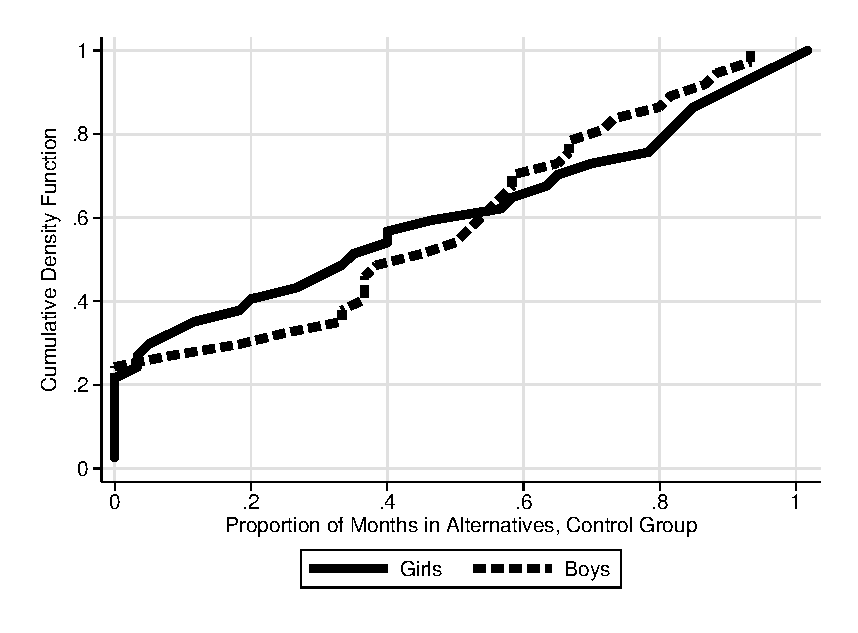
\includegraphics[width=\textwidth]{output/abccare_controlcontamination_boysgirls}
\end{subfigure}%
\begin{subfigure}[h]{0.4\textwidth}
	\centering
	\caption{Socioeconomic Disadvantage by Gender} \label{figure:disadgender}
	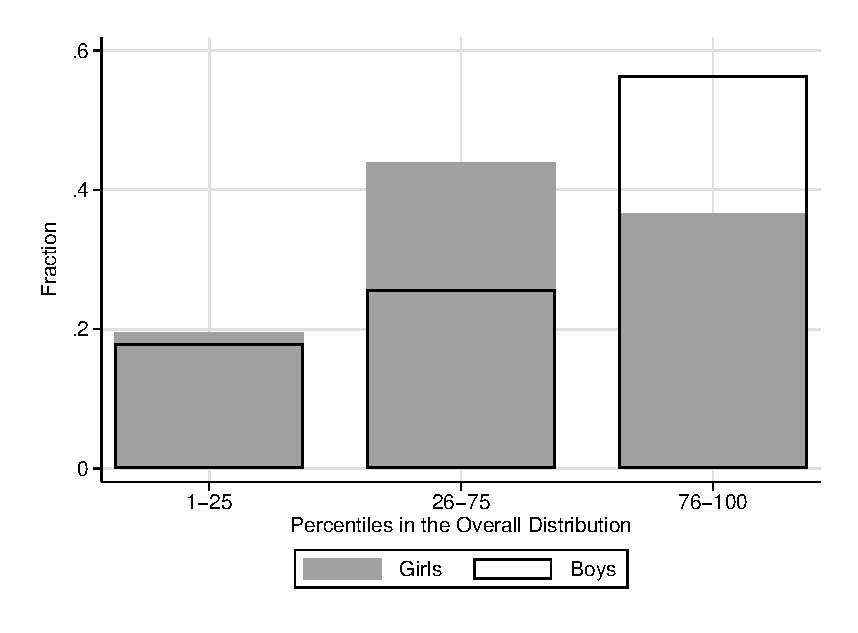
\includegraphics[width=\textwidth]{output/factorbase_girlsboyscompare}
\end{subfigure}
\begin{subfigure}[h]{0.4\textwidth}
	\centering
	\caption{Disadvantage by Take-up of Alternatives, Girls} \label{figure:disadgirls}
	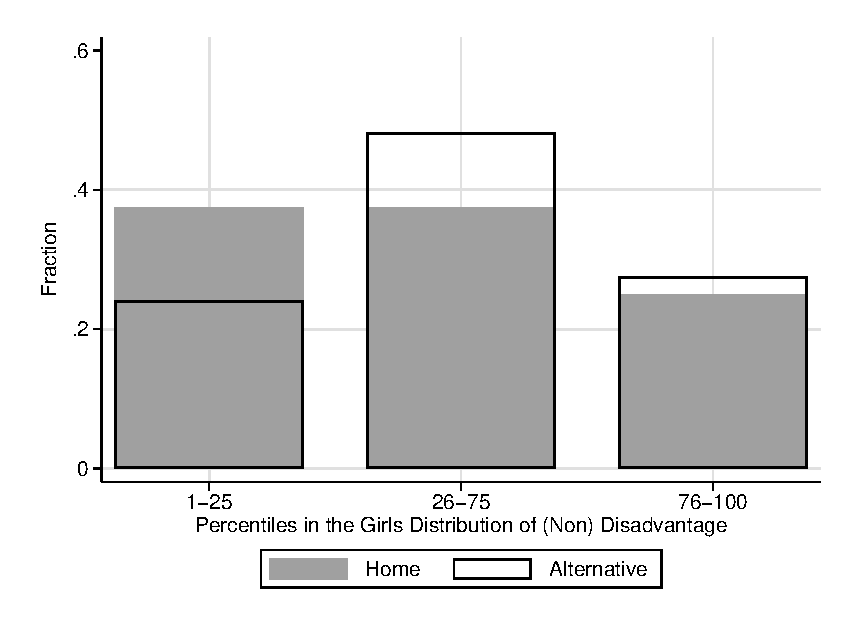
\includegraphics[width=\textwidth]{output/factorbase_wgirlscompare}
\end{subfigure}%
\begin{subfigure}[h]{0.4\textwidth}
	\centering
	\caption{Disadvantage by Take-up of Alternatives, Boys} \label{figure:disadboys}
	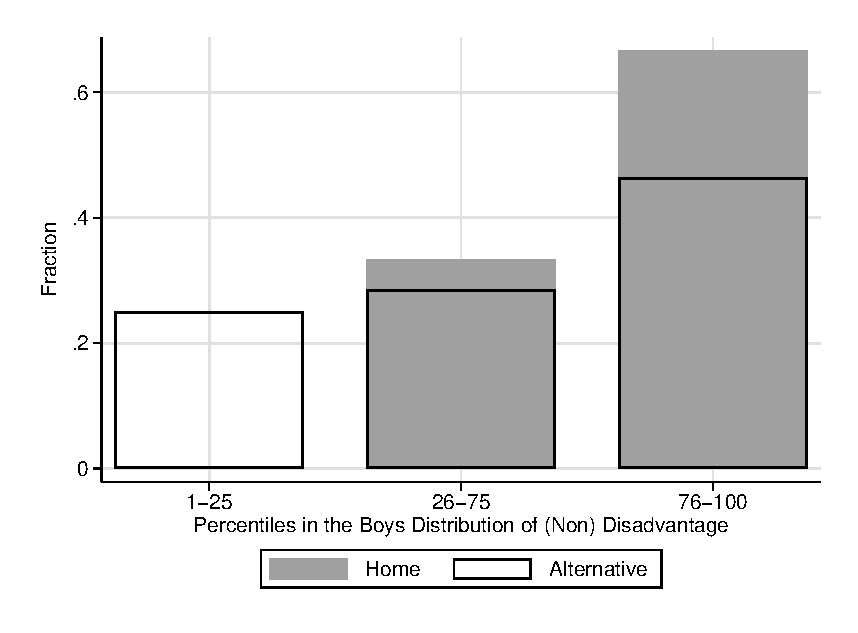
\includegraphics[width=\textwidth]{output/factorbase_wboyscompare}
\end{subfigure}
\footnotesize
\justify
\textbf{Note:} Panel (a) displays the cumulative distribution function of enrollment in alternatives by gender. Panel (b) displays how girls and boys separately fit into the overall (girls and boys pooled) distribution of socioeconomic disadvantage. Panel (c) displays how girls who did not enroll and enrolled in alternatives fit into the overall girls distribution of socioeconomic disadvantage. Panel (d) is analogous to Panel (c) for boys. Our measure of socioeconomic disadvantage is a latent or a factor of the following variables: Mother's age, education, IQ, marital status, and employment, as well as number of children and father's presence at home.
\end{sidewaysfigure}

A better understanding of the counterfactual scenario that children would faced if not in ABC/CARE is useful in explaining the gender differences in the treatment effects. This requires us to identify the parameter in Equation~\eqref{eq:cont1}: The comparison between treatment and staying at home. It also requires us to identify the parameter in Equation~\eqref{eq:cont2}: The analogous comparison to children who attended alternative preschools. These parameters are not identified by randomization into treatment or control. The parents of the control-group children selected either to keep their children at home or take them to preschool alternatives that were available when ABC/CARE was implemented. 

We rely on econometric methods for identification. In the main text, we rely on matching.\footnote{See \citet{Heckman_Ichimura_etal_1998_REStud} for a general discussion of the method, and an assessment of its practical implementation.} This method is practical in our case due to the small size of our samples. In Appendix~\ref{}, we show that instrumental-variable and control-function methods yield similar results but lack precision. In Appendix~\ref{}, we discuss and document our choice of the matching variables, as well as other practical aspects of the implementation of this estimator.

Column (3) shows the raw difference between the treatment-group children and the control-group children who stayed at home. Column (4) implements a matching estimator to weight this difference and fix the counterfactual to ``staying at home.''  Columns (5) and (6) are analogous when fixing the counterfactual to attending an alternative preschool. A clear pattern emerges: Girls benefit more from treatment if compared to staying at home, while boys benefit more from treatment is compared to alternative preschools. For example, \textbf{[JLG: discussion on magnitudes here once Josh factors are available.]} Tables~\ref{table:massiveall1} and~\ref{table:massiveall2} corroborate this when using our different methodologies to assess treatment effects across categories. \textbf{[JLG: discussion on magnitudes here once these two tables are available.]}

\textbf{[JLG: place the two massive all tables here (counterfactual comparisons).]}

The sharp difference in the comparison of treatment to staying at home and alternative preschools suggests that boys and girls faced different situations of socio-economic disadvantaged at home. Figure~\ref{figure:socdis} investigates this. We start by noting that take-up of alternatives does not differ by gender (Panel~\ref{figure:altgender}). What differs by gender is socioeconomic disadvantage. We create a measure of socioeconomic disadvantage at baseline creating a latent or a factor of the following variables: Mother's age, education, IQ, marital status, and employment, as well as number of children and father's presence at home. We assess how girls and boys fit into the overall distribution of this latent in the control group. Boys are disproportionately more advantaged than girls (Panel~\ref{figure:disadgender}).\footnote{Note that this measure is based on baseline characteristics, so this result holds for the treatment group.} This means that girls in the control group were taken care in a disadvantaged environment or went to the lowest quality preschools because their families were more resource constrained if compared to their boy counterparts. Thus, they benefited more than boys if compared to the next best  alternative as perceived by their parents, as documented in Section~\ref{sec:treatment-effects}.

We formally test the difference in disadvantaged across boys and girls in Table~\ref{table:disadtests}. We reject the null of a common joint distribution of the variables composing our measure of socioeconomic disadvantage across girls and boys (at baseline). Panels~\ref{figure:disadgirls} and~\ref{figure:disadboys} of Figure~\ref{figure:socdis} we further dissect socioeconomic disadvantage within genders, and provide the corresponding tests in Table~\ref{table:disadtests}. 

Parents of relatively more advantaged girls are sent to preschool alternatives more often. Parents of relatively more advantaged boys are sent to preschool alternatives more often. This provides an explanation why girls benefited more from treatment if compared to staying at home---which would be a more disadvantaged environment to develop if compared to their male counterparts, while boys benefited more from treatment if compared to attending alternatives---which would be relatively worst given that their parents plausibly sent them to worst alternatives due to a lack of resources or were worst complements to those learning environments. 

\begin{table}[!htpb]
\begin{threeparttable}
\caption{Gender and Baseline Socioeconomic Disadvantage in the Control Group, Tests} \label{table:disadtests}
\centering 
\begin{tabularx}{16.5cm}{XcX}
& \begin{tabular}{cccc}
\toprule
Males vs. Females & & \mc{2}{c}{Alt. vs. Home} \\
\cmidrule(lr){1-2} \cmidrule(lr){3-4}
Control Group & & Males & Females \\
\midrule
\textbf{0.007} & & \textbf{0.006} & 0.110 \\
\bottomrule
\end{tabular}

% Control, males vs. females: distance between: factor of m_age_base, m_ed_base, m_iq_base, hh_sibs_base, hrabc_index

% Alt. vs home: factor of m_age_base, m_ed_base, m_iq_base, hh_sibs_base, hrabc_index & 
\end{tabularx}
\begin{tablenotes}
\footnotesize
\item \textbf{Note:} This table the null of a common joint distribution of the variables composing our measure of socioeconomic disadvantage (mother's age, education, IQ, marital status, and employment, as well as number of children and father's presence at home) between males and females in the control group and between children who attended  alternative preschool and who stayed at home (within control-group boys or within control-group girls). The $p$-values are asymptotic following \citet{Rosenbaum_2005_Distribution_JRSS}. Statistics significant at the $0.10$ level are bolded.
\end{tablenotes}
\end{threeparttable}
\end{table}










